 % This must be in the first 5 lines to tell arXiv to use pdfLaTeX, which is strongly recommended.
\pdfoutput=1
% In particular, the hyperref package requires pdfLaTeX in order to break URLs across lines.

\documentclass[11pt]{article}

\usepackage[review]{EMNLP2023}

% Standard package includes
\usepackage{times}
\usepackage{latexsym}

% For proper rendering and hyphenation of words containing Latin characters (including in bib files)
% \usepackage[T1]{fontenc}
% For Vietnamese characters
% \usepackage[T5]{fontenc}
% See https://www.latex-project.org/help/documentation/encguide.pdf for other character sets

% This assumes your files are encoded as UTF8
% \usepackage[utf8]{inputenc}
\usepackage[T5]{fontenc}
\usepackage[utf8]{inputenc}

% \usepackage{multicol}
\usepackage{pdfpages}
% \BLOCK{if not nopax}
% \usepackage{pax}
% \BLOCK{endif}
% \usepackage{times}
% \usepackage[english,latin]{babel}

% This is not strictly necessary and may be commented out.
% However, it will improve the layout of the manuscript,
% and will typically save some space.
\usepackage{microtype}

% This is also not strictly necessary and may be commented out.
% However, it will improve the aesthetics of text in
% the typewriter font.
\usepackage{array}
\usepackage{inconsolata}
\usepackage{amsmath}
\usepackage{multirow}
\usepackage{graphicx}
\usepackage{arydshln}
\usepackage{fdsymbol}
\usepackage{ifsym}
\usepackage{tablefootnote}
\usepackage{tikz}
\usepackage{wasysym}
\usepackage{booktabs} 
\usepackage{algorithm}
\usepackage{longtable}
\usepackage{subcaption}
\usepackage{etoolbox}
\usepackage{caption}
\usepackage{lipsum}


% If the title and author information does not fit in the area allocated, uncomment the following
%
\setlength\titlebox{6.25cm}
%
% and set <dim> to something 5cm or larger.

\title{Project Report: Titanic - Machine Learning from Disaster}

\author{
Trần Nguyễn Tuấn Anh, Nguyễn Phú Hào, Lê Tấn Hoà\\
Khoa Khoa học và Kỹ thuật thông tin, Trường Đại học Công nghệ Thông tin \\
Công nghệ Thông tin định hướng Nhật Bản, Trường Đại học Công nghệ Thông tin \\
Đại học Quốc gia Thành phố Hồ Chí Minh \\
\texttt{\{21521840, 21520223, 21522081\}@gm.uit.edu.vn}
}
\microtypesetup{protrusion=false}
\begin{document}

\maketitle

\begin{abstract}
Đồ án này tập trung vào việc phân tích dữ liệu của hành khách trên tàu Titanic, sử dụng bộ dữ liệu được cung cấp trên Kaggle. Mục tiêu chính là xây dựng mô hình dự đoán khả năng sống sót của hành khách dựa trên các thông tin như giới tính, lớp hành khách, tuổi tác và các đặc trưng khác. Qua quá trình khám phá dữ liệu và tiền xử lý, chúng tôi đã tìm hiểu về đặc trưng và ảnh hưởng của chúng đối với khả năng sống sót. Sau đó, chúng tôi đã triển khai một số mô hình học máy như Random Forest và Support Vector Machine để dự đoán sống sót trên tập huấn luyện. Kết quả được đánh giá thông qua các phương pháp đánh giá hiệu suất Accuracy. Đồ án này không chỉ giúp hiểu rõ hơn về các đặc trưng quyết định sống sót trên tàu Titanic mà còn thể hiện quá trình triển khai mô hình học máy để dự đoán trong tình huống tương tự.
\end{abstract}

\section{Exploratory Data Analysis}
Tập dữ liệu Titanic bao gồm thông tin về hành khách và thủy thủ đoàn trên tàu Titanic, bao gồm tên, tuổi, giới tính, địa điểm sinh, địa điểm lên tàu, lớp vé, giá vé, v.v. Tập dữ liệu huấn luyện ( tập train) có 891 hàng và 11 cột. Trong khi đó, tập kiểm thử (tập test) chỉ có 418 hàng và 11 cột. Dữ liệu Titanic bao gồm cả dữ liệu định tính (Categorical Data) và dữ liệu định lượng (Numerical Data). Dữ liệu định tính bao gồm các cột như Pclass, Survived, Embarked, Pclass, Sibsp, Parch. Dữ liệu định lượng bao gồm các cột như Age, Fare. Ngoài ra, có một số giá trị thiếu trong tập dữ liệu Titanic. Các cột có giá trị thiếu bao gồm Age, Fare, Cabin, Embarked.\\
Từ tập dữ liệu, chúng tôi đã phân tích được một số đặc trưng. Sau khi huấn luyện dữ liệu, chúng tôi nhận thấy, số người sống sót là 342 người, trong khi đó, 549 người chết, Tỷ lệ sống sót trung bình của hành khách trên tàu Titanic là 38.4\%.

% Example:
\begin{figure}[ht]
    \centering
    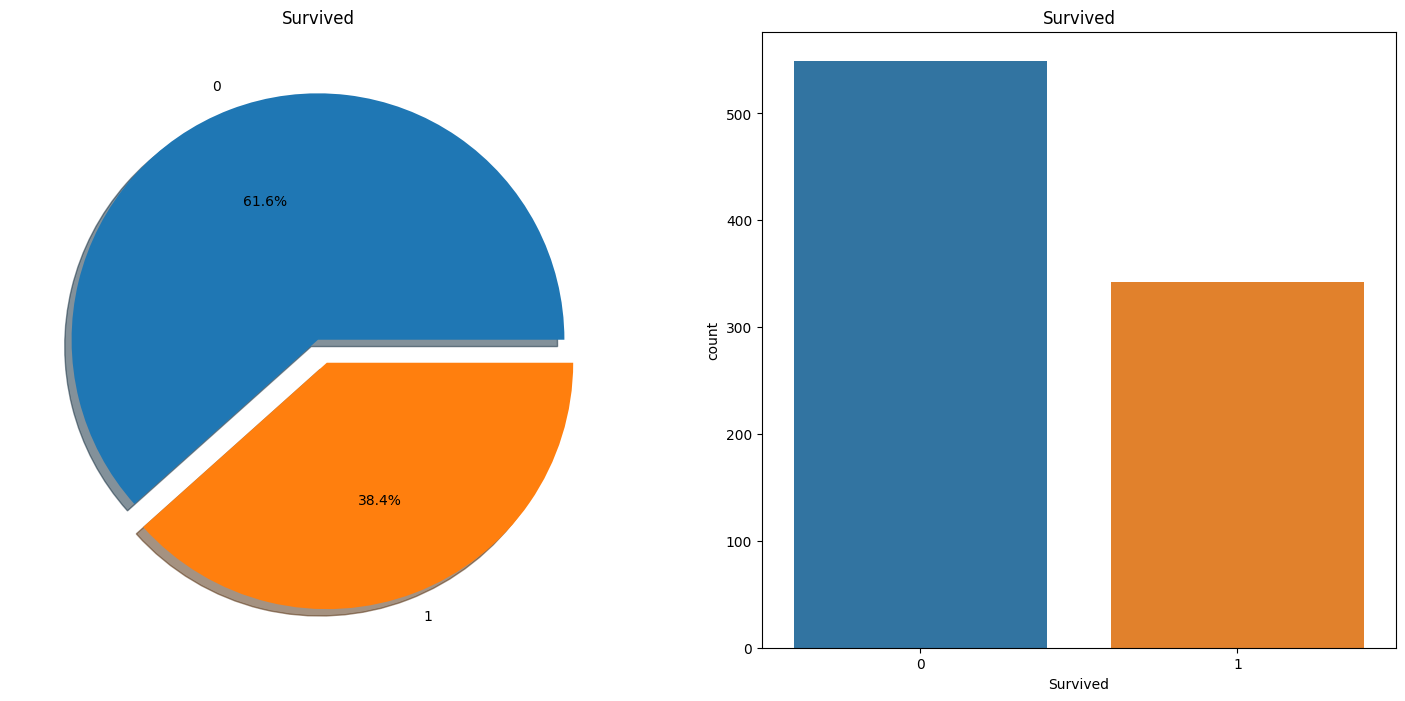
\includegraphics[width=\columnwidth]{titanicreport/figs/fig1.png}
    \caption{Khả năng sống sót của hành khách trên tàu Titanic.}

\end{figure}
Về  đặc trưng giới tính (Sex), chúng tôi nhận thấy, số lượng nam giới tử vong  là 577 người, trong khi đó, 314 nữ giới. Tỷ lệ tử vong của hành khách trên tàu Titanic theo giới tính lại có sự chênh lệch. Phụ nữ có tỷ lệ sống sót cao hơn nam giới, với 65\% so với 35\%.Điều này có thể được giải thích bởi một số yếu tố, bao gồm: Phụ nữ và trẻ em được ưu tiên lên thuyền cứu sinh. Phụ nữ có thể dễ dàng tìm kiếm sự giúp đỡ hơn nam giới.Kết quả này cho thấy rằng giới tính là một yếu tố quan trọng ảnh hưởng đến khả năng sống sót của hành khách trên tàu Titanic.\\
% Example:
\begin{figure}[ht]
    \centering
    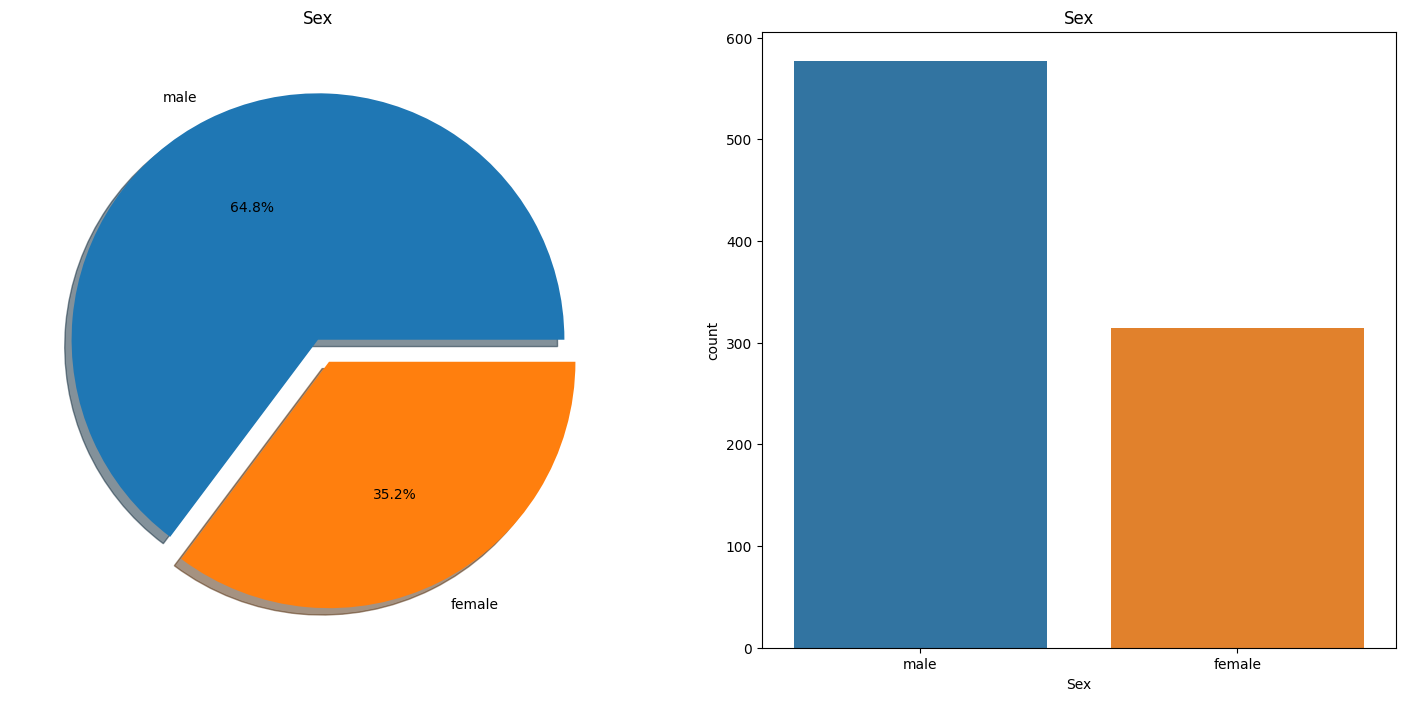
\includegraphics[width=\columnwidth]{titanicreport/figs/fig2.png}
    \caption{Tỷ lệ tử vong của hành khách đựa vào đặc trưng .}
 
\end{figure}
Đặc trưng nơi hành khách lên tàu (Embarked), cho thấy rằng hành khách ở khu vực Southampton có tỷ lệ tử vong cao hơn 72.4\%, hành khách ở khu vực Queenstown (8.7\%) và Cherbourg (18.9\%). Điều này có thể được giải thích bởi một số yếu tố, bao gồm: Hành khách ở khu vực Southampton thường có địa vị xã hội cao hơn hành khách ở khu vực Queenstown và Cherbourg. Hành khách ở khu vực Southampton thường có sức khỏe tốt hơn hành khách ở khu vực Queenstown và Cherbourg. Đây là một yếu tố tác động gián tiếp đến khả năng sống sót của hành khách.\\
% Example:
\begin{figure}[ht]
    \centering
    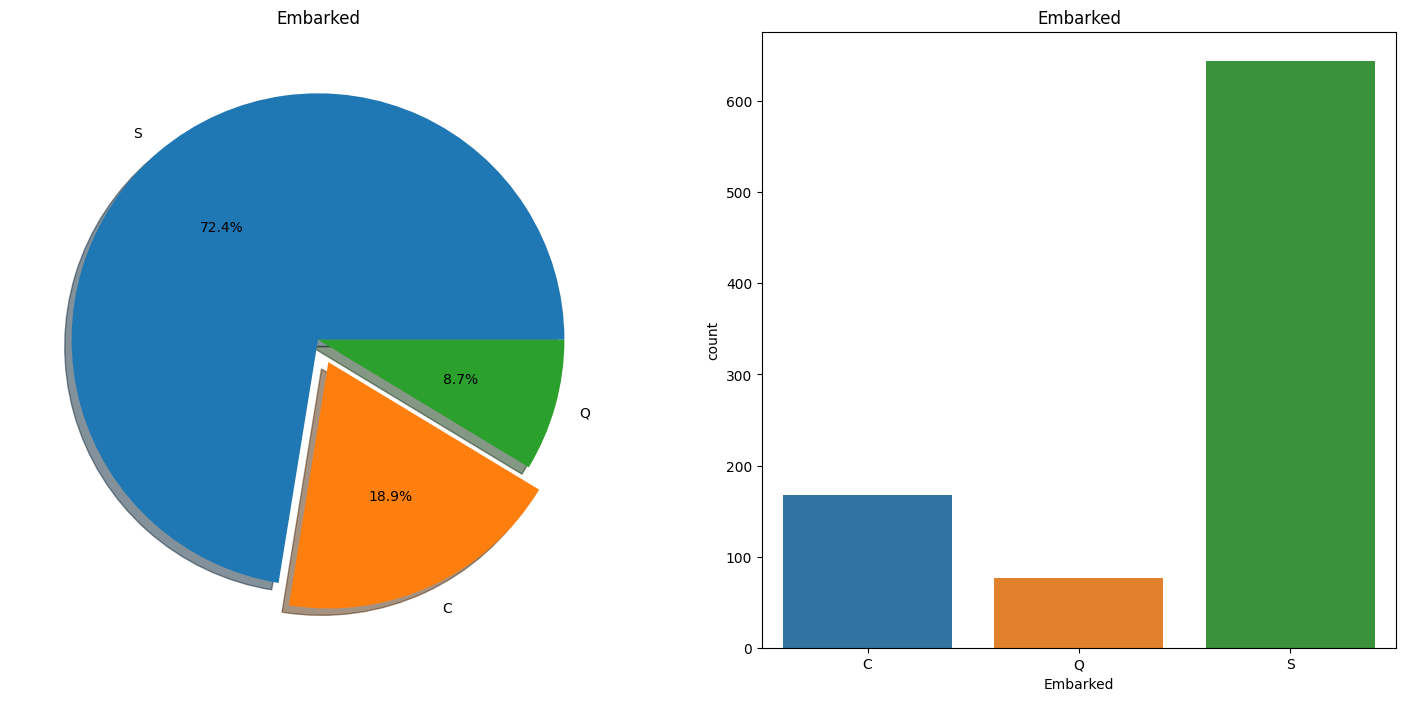
\includegraphics[width=\columnwidth]{titanicreport/figs/fig3.png}
    \caption{Tỷ lệ tử vong của hành khách đựa vào đặc trưng nơi hành khách lên tàu.}
    
\end{figure}
Đối với đặc trưng hạng vé (Pclass), tỷ lệ sống sót của hành khách trên tàu Titanic theo hạng vé. Hành khách ở hạng vé 3 có tỷ lệ tử vong cao nhất, với 55.1\%. Hành khách ở hạng vé 2  và thứ 1 có tỷ lệ tử vong thấp nhất, với 20.7\% và 24.2\%.Điều này có thể được giải thích bởi một số yếu tố, bao gồm:Hành khách ở hạng vé nhất thường có địa vị xã hội cao hơn và được ưu tiên lên thuyền cứu sinh.Hành khách ở hạng vé nhất thường có sức khỏe tốt hơn và có khả năng sống sót trong điều kiện khắc nghiệt.Kết quả này cho thấy rằng hạng vé là một yếu tố quan trọng ảnh hưởng đến khả năng sống sót của hành khách trên tàu Titanic.\\
% Example:
\begin{figure}[ht]
    \centering
    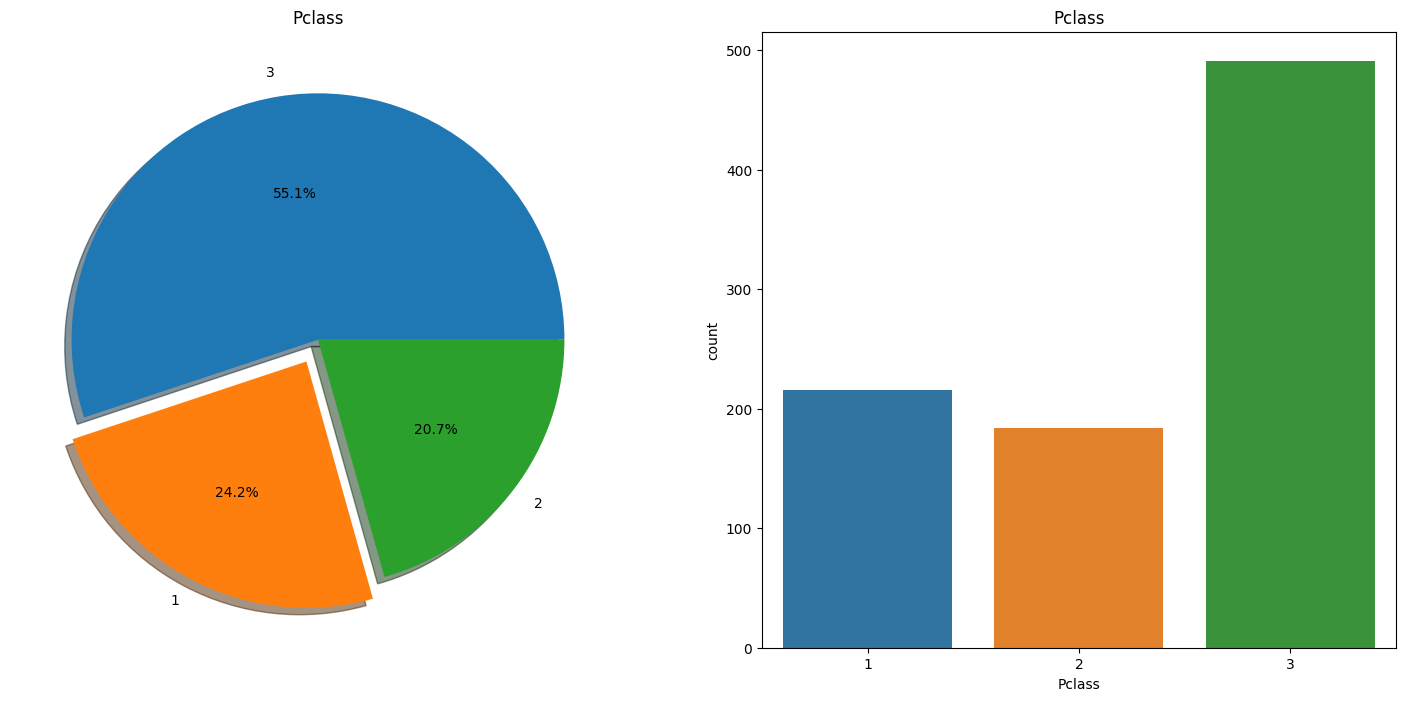
\includegraphics[width=\columnwidth]{titanicreport/figs/fig4.png}
    \caption{Tỷ lệ tử vong của hành khách đựa vào đặc trưng Hạng vé.}
 
\end{figure}
Còn các đặc trưng SibSp,Parch tác động không đáng kể đến khả năng sống sót của hành khách trên tàu Titanic. Đối với đặc trưng Parch, tỷ lệ tử vong cao ở những hành khách đi một mình với 76.1\%, tỷ lệ tử vong giảm dần với các hành khác đi cùng 1, 2 hoặc nhiều thành viên trong gia đình.  HÌnh~\ref{fig:feature} trình bày khả năng sống sốt (tỷ lệ sống sót) của hành khách trên tàu Titanic dựa trên các đặc trưng của tập dữ liệu.\\
% Example:
\begin{figure}[t]
    \centering
    \begin{subfigure}{0.48\textwidth}
        \centering
        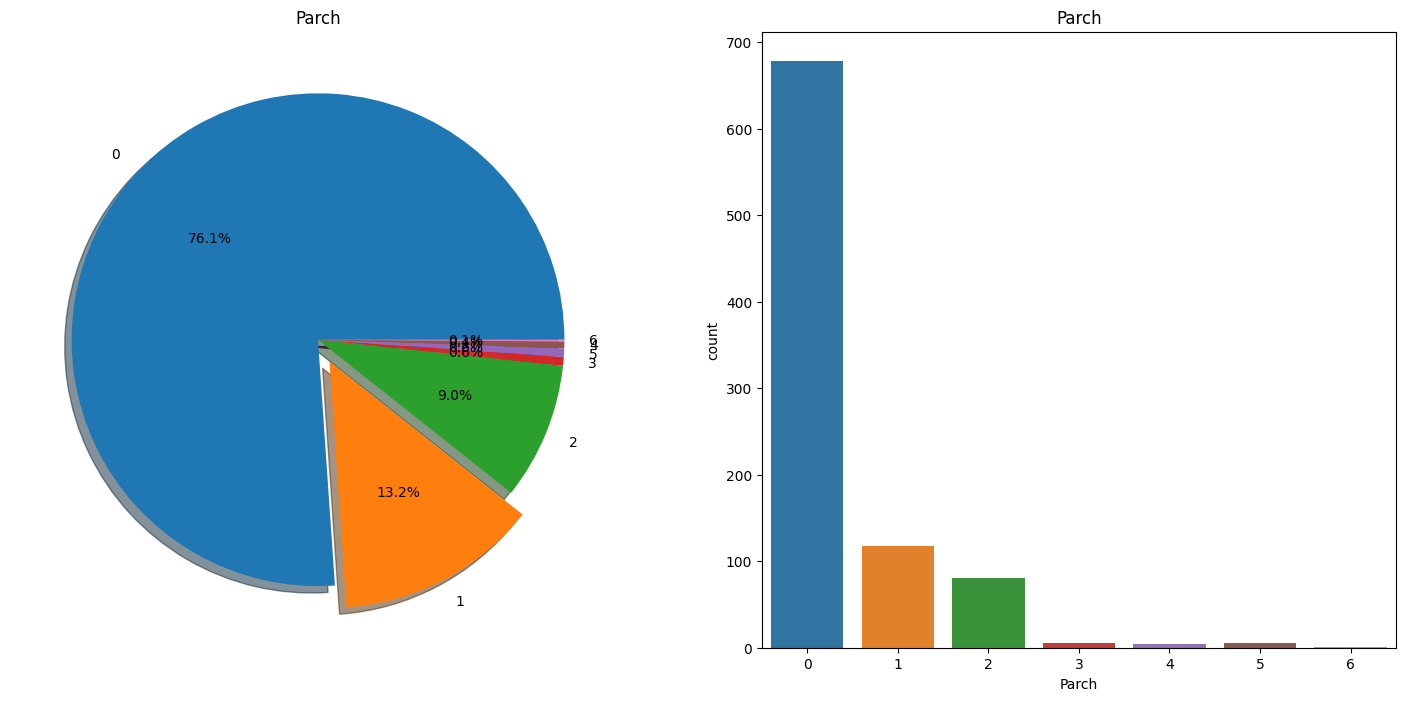
\includegraphics[width=\textwidth]{titanicreport/figs/fig5.png}
        \caption{Tỷ lệ tử vong của hành khách đựa vào đặc trưng Số lượng ba mẹ con cái đi cùng.}
        
    \end{subfigure}
    \hfill
    \begin{subfigure}{0.48\textwidth}
        \centering
        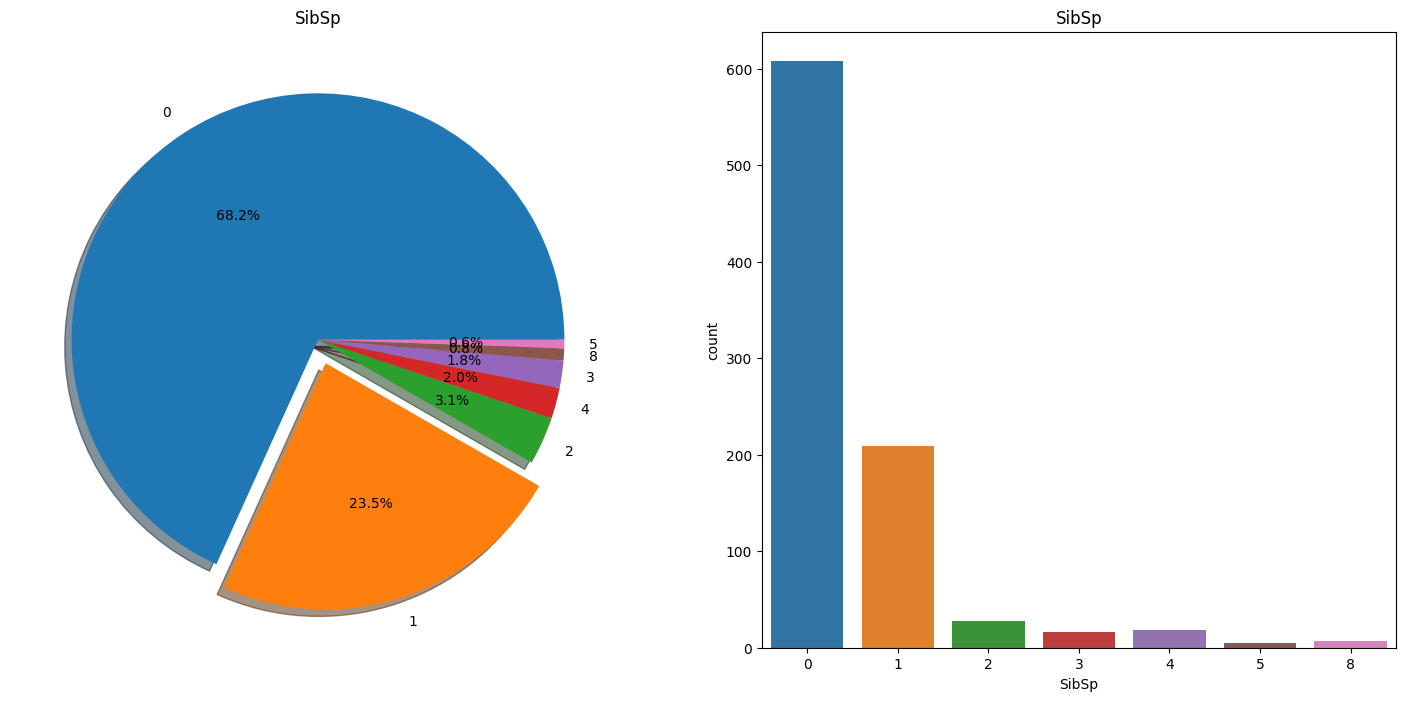
\includegraphics[width=\textwidth]{titanicreport/figs/fig6.png}
        \caption{Tỷ lệ tử vong của hành khách đựa vào đặc trưng Số lượng vợ chồng, anh em đi cùng.}
      
    \end{subfigure}
    \caption{Tỷ lệ tử vong của hành khách đựa vào đặc trưng số lượng thành viên trong Gia đình.}
\end{figure}
Ngoài ra, chúng tôi nhân thấy dữ liệu định lượng bao gồm các cột như Age, Fare cũng có ảnh hưởng đáng kể đến tỷ lệ tử vong của hành khách trên tàu Titanic. Đầu tiên, ở cột 'Age' chúng tôi trực quan hóa phân phối tuổi bằng biểu đồ Histogram  hình~\ref{fig:fare} hiển thị phân phối tuổi của hành khách trên tàu Titanic. Phân phối tuổi có dạng hình chuông, với đỉnh ở khoảng 29 tuổi. Điều này cho thấy rằng phần lớn hành khách là thanh niên trưởng thành.Có một số điểm nổi bật đáng chú ý trong phân phối tuổi:\\
\begin{itemize}
    \item Tỷ lệ hành khách trẻ em (dưới 10 tuổi) là tương đối cao.
    \item Tỷ lệ hành khách cao tuổi (60 tuổi trở lên) là tương đối thấp.
    \item Tỷ lệ hành khách ở độ tuổi trung niên (30-59 tuổi) là cao nhất.
\end{itemize}
Dựa vào sự phân phối độ tuổi có thể được sử dụng để hiểu rõ hơn về thảm họa Titanic. Ví dụ, tỷ lệ sống sót của trẻ em cao hơn tỷ lệ sống sót của người lớn. Điều này có thể là do trẻ em được ưu tiên lên thuyền cứu sinh.
Tiếp theo, chúng tôi nhận thấy đặc trưng giá vé 'Fare' có ảnh hưởng đáng kể đến tỷ lệ tử vong của hành khách trên tàu Titanic. Chúng tôi trực qua hoá phân phối giá vé của hành khách trên tàu Titanic bằng biểu đồ Histogram hình~\ref{fig:age} phân bố giá vé không tuân theo phân bố chuẩn, mà nghiêng về bên trái (nhiều hành khách mua vé rẻ hơn). với đỉnh ở khoảng £30. Điều này cho thấy rằng phần lớn hành khách mua vé rẻ hơn. Có một số điểm nổi bật đáng chú ý trong phân phối giá vé:
\begin{itemize}
    \item Tỷ lệ hành khách mua vé rẻ hơn (dưới £50) là tương đối cao.
    \item Tỷ lệ hành khách mua vé đắt hơn (£50 trở lên) là tương đối thấp.
\end{itemize}
Nhìn chung, giá vé là một đặc trưng quan trọng trong tập dữ liệu Titanic. Nó cung cấp thông tin về nhiều khía cạnh khác nhau của thảm họa, bao gồm: Tầng lớp kinh tế của hành khách, cơ hội sống sót của hành khách, mối quan hệ giữa các biến khác nhau.
\begin{figure}[ht]
    \centering
    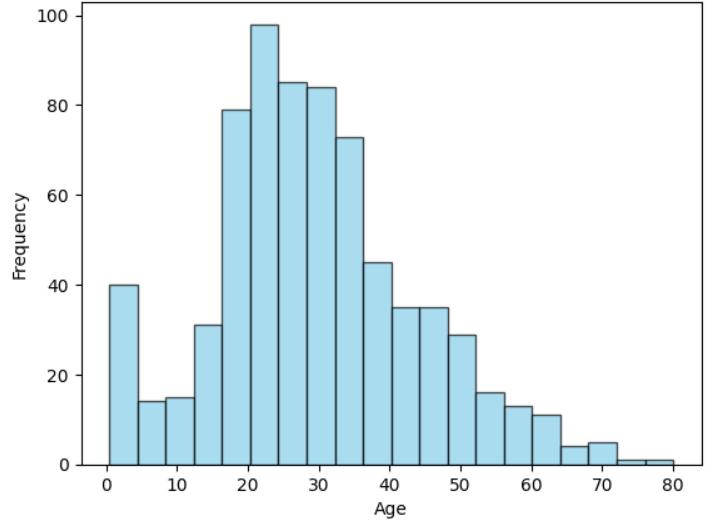
\includegraphics[width=\columnwidth]{titanicreport/figs/fig10.png}
    \caption{Tỷ lệ tử vong của hành khách đựa vào độ tuổi.}
    \label{fig:age}
\end{figure}
\begin{figure}[ht]
    \centering
    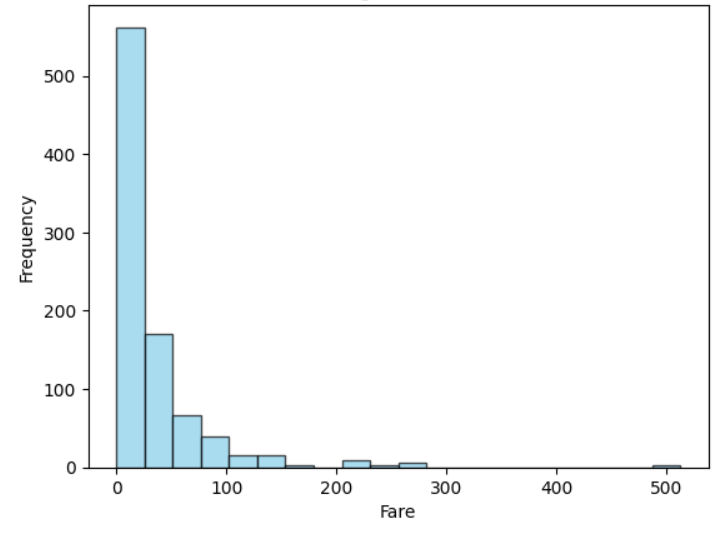
\includegraphics[width=\columnwidth]{titanicreport/figs/fig11.png}
    \caption{Tỷ lệ tử vong của hành khách đựa vào giá vé tàu.}
     \label{fig:fare}
\end{figure}
\begin{figure*}[ht]
    \centering
    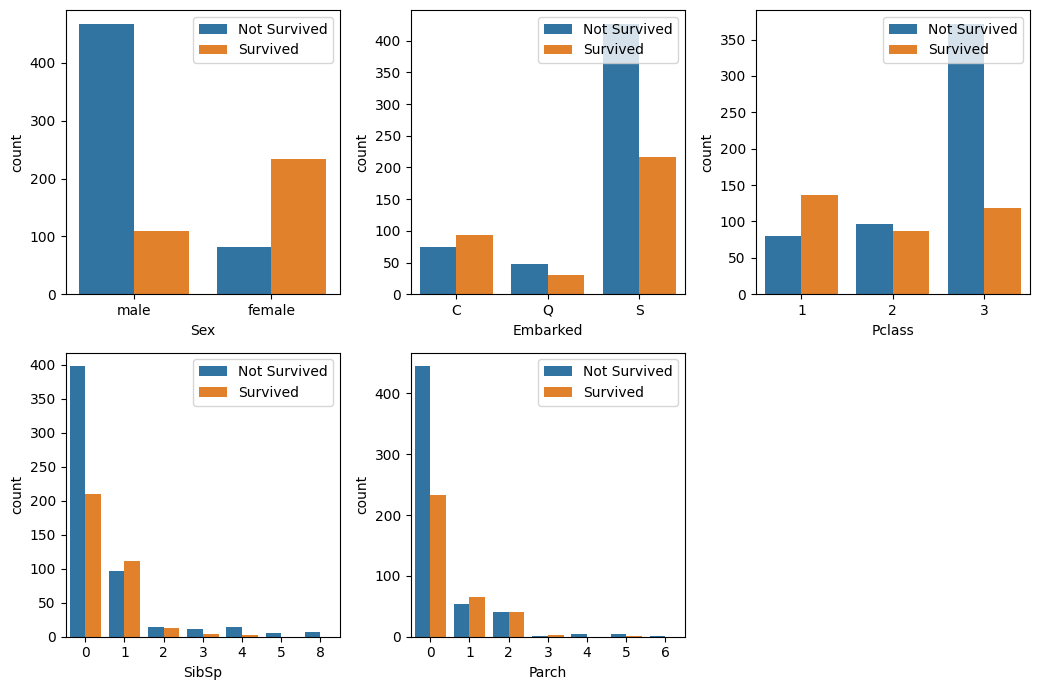
\includegraphics[width=\textwidth]{titanicreport/figs/fig7.png}
    \caption{Tỷ lệ tử vong của hành khách đựa vào categorical data.}
    \label{fig:feature}
\end{figure*}

\section{Data Preprocessing}
Quá trình chuẩn bị dữ liệu cho phân tích và mô hình hóa bao gồm các bước như làm sạch dữ liệu, loại bỏ các giá trị ngoại lai, chuyển đổi kiểu dữ liệu, và tạo các tính năng mới.Trong bước này, nhóm thực hiện 2 bước, trong đó gồm nhiều xử lí nhỏ gồm: Feature Engineering và Data Wrangling.
\subsection{Feature Engineering}
Để tiến hành phân tích và mô hình hóa tập dữ liệu, trước tiên cần thực hiện quá trình \textit{Feature Engineering}, bước này liên quan đến việc tạo ra các tính năng mới từ các tính năng hiện có. Điều này có thể giúp cải thiện độ chính xác và hiệu suất của các mô hình.Trong bước này, nhóm thực hiện xử lí, tạo dữ liệu dựa trên 5 cột khác nhau: Name, Ticket, Sibsp, Parch, Age.\\
% Example:
Đầu tiên, chúng tôi nhận thấy cột ‘Name’ có thể trích xuất (extract) danh hiệu (như "Miss", "Mr", "Mrs", "Dr", v.v.) từ các tên đầy đủ trong một tập dữ liệu và tạo một cột mới có tên 'Title' để lưu trữ các danh hiệu đã trích xuất. Hàm \texttt{extract\_title} sẽ trích xuất danh hiệu từ mỗi tên. Chẳng hạn, nếu có một tên 'Smith, Miss. Jane Marie' trong cột 'Name', sau khi thực thi dòng mã này, cột 'Title' sẽ chứa giá trị 'Miss' tương ứng với tên đó. Tiếp theo, chúng tôi tiến hành nhóm các danh hiệu thành các danh mục phổ biến và xử lý các danh hiệu ít phổ biến hơn. Áp dụng hàm \texttt{group\_title} cho từng danh hiệu trong cột 'Title' của DataFrame và cập nhật cột đó với kết quả nhóm danh hiệu.
\textbf{Ví dụ:}
\begin{itemize}
    \item Nếu danh hiệu ban đầu là 'Mr', 'Mrs', 'Miss' hoặc 'Master', nó sẽ giữ nguyên.
    \item Nếu danh hiệu ban đầu là 'Ms', nó sẽ được chuyển thành 'Miss'.
    \item Nếu danh hiệu ban đầu là 'Dr', 'Rev', 'Col', v.v., nó sẽ được chuyển thành 'Others'.
\end{itemize}
\begin{table}[htbp]
\centering
\caption{Danh hiệu các hành khách trong cột Name}
\label{tab:passengers_small}
\begin{tabular}{|c|c|p{0.4\columnwidth}|}
\hline
\multicolumn{1}{|c|}{\textbf{PassengerID}} & \multicolumn{1}{c|}{\textbf{Pclass}} & \multicolumn{1}{c|}{\textbf{Name}} \\ \hline
892 & 3 & Kelly, Mr. James \\ \hline
893 & 3 & Wilkes, Mrs. James (Ellen Needs) \\ \hline
894 & 2 & Myles, Mr. Thomas Francis \\ \hline
895 & 3 & Wirz, Mr. Albert \\ \hline
896 & 3 & Hirvonen, Mrs. Alexander (Helga E Lindqvist) \\ \hline
897 & 3 & Svensson, Mr. Johan Cervin \\ \hline
898 & 3 & Connolly, Miss. Kate \\ \hline
899 & 2 & Caldwell, Mr. Albert Francis \\ \hline
900 & 3 & Abrahim, Mrs. Joseph (Sophie Halaut Easu)... \\ \hline
\end{tabular}
\end{table}


Việc trích xuất danh hiệu cũng như nhóm các danh hiệu hữu ích cho quá trình phân tích và mô hình hóa ở các bước sau này. Chúng tôi sẽ khám phá mối quan hệ giữa danh hiệu hành khách và kết quả sống sót trên tàu Titanic.\\
Chúng tôi sẽ sử dụng biểu đồ đếm Seaborn để trực quan hóa phân phối của những người sống sót và không sống sót trên các danh hiệu khác nhau, cung cấp những hiểu biết về các mẫu và xu hướng tiềm ẩn. Thông qua hình~\ref{fig:title} Biểu đồ cho thấy tỷ lệ sống sót của hành khách trên tàu Titanic theo danh hiệu. Có thể thấy rằng, tỷ lệ sống sót của phụ nữ cao hơn đáng kể so với nam giới. Cụ thể, tỷ lệ sống sót của phụ nữ với danh hiệu 'Mrs' và 'Miss' lần lượt là 74,2\% và 85,8\%, trong khi tỷ lệ sống sót của nam giới với danh hiệu 'Mr' chỉ là 18,9\%.

\begin{figure}[ht]
    \centering
    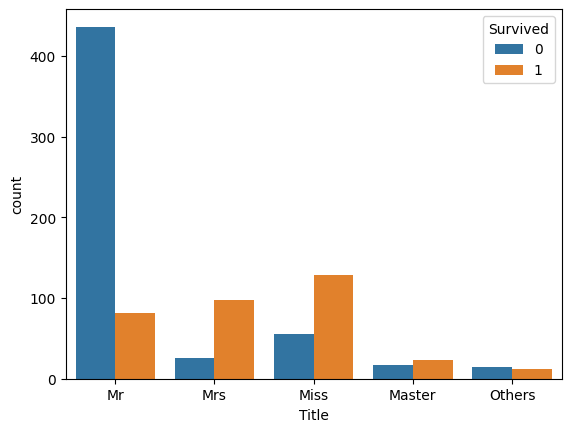
\includegraphics[width=\columnwidth]{titanicreport/figs/fig8.png}
    \caption{Tỷ lệ sống sót của hành khách trên tàu Titanic theo danh hiệu.}
    \label{fig:title}
\end{figure}
% Example:
Tiếp theo, chúng tôi nhận thấy cột 'Ticket'  chứa nhiều giá trị du nhập ( mỗi hành khách có một mã vé riêng), dữ liệu mang tính chất phi hiện hữu ( sử dụng trực tiếp không mang lại ý nghĩa) cho nên cần xử lý dữ liệu bằng cách giảm chiều dữ liệu, tạo ra các giá trị tiền tố chung để thể hiện nhóm hoặc loại hành khách.
\begin{figure}[ht]
    \centering
    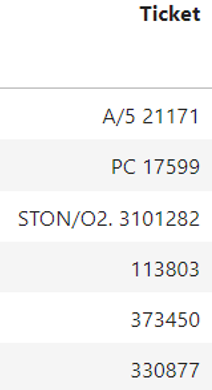
\includegraphics[width=0.5\columnwidth]{titanicreport/figs/ticket.png}
    \caption{Các loại vé trong cột Ticket}
\end{figure}
Điều này có thể giúp mô hình hóa dữ liệu hiệu quả hơn. Cột 'Ticket' có thể cung cấp thêm thông tin về hành khách, như loại vé, nhóm hoặc vùng lên tàu. Việc xử lý có thể giúp chúng ta chiết xuất thông tin này và sử dụng nó trong mô hình hóa. Qua đó, việc xử lý cột 'Ticket' giúp làm sạch và rút gọn dữ liệu, làm cho nó phù hợp hơn để áp dụng vào các mô hình học máy và phân tích. Quá trình xử lý dữ liệu cột 'Ticket' được tiến hành tương tự như xử lý cột 'Name'.Đầu tiên, chúng tôi loại bỏ các ký tự không phải là chữ số khỏi cột "Ticket" và chỉ giữ lại các chữ số đầu tiên của giá trị.Hàm replace() được sử dụng để thay thế tất cả các ký tự không phải là chữ số trong cột "Ticket" bằng ký tự trống. Các tiền tố của các giá trị không phải số được giữ lại, và giá trị số được thay thế bằng "X".Hàm \texttt{split()} được sử dụng để tách giá trị của cột "Ticket" thành các phần dựa trên dấu chấm hoặc dấu gạch chéo.Phần đầu tiên của giá trị được lưu trữ trong mảng Ticket. Mảng Ticket được chuyển đổi thành một chuỗi và được sử dụng để thay thế giá trị của cột "Ticket".Sau khi thực hiện, cột "Ticket" sẽ chỉ chứa các tiền tố của giá trị ban đầu. Điều này sẽ đơn giản hóa dữ liệu và giúp phân tích dễ dàng hơn. Tiếp theo, dùng hàm \texttt{group\_ticket}nhóm các hành khách có cùng loại vé lại với nhau. Sử dụng phương thức \texttt{apply} kết hợp với hàm \texttt{lambda} để áp dụng hàm \texttt{group\_ticket} cho từng giá trị trong cột 'Ticket' của tập dữ liệu huấn luyện \texttt{(train\_df)} và kiểm tra \texttt{(test\_df)}.Kết quả là cột 'Ticket' đã được cập nhật với các giá trị mới được nhóm. Qua việc xử lý dữ liệu cột 'Ticket', chúng tôi đã tạo ra feature mới có thể được sử dụng để phân tích xem loại vé có ảnh hưởng đến khả năng sống sót của hành khách hay không. Ví dụ, nếu các hành khách có vé hạng cao có tỷ lệ sống sót cao hơn các hành khách có vé hạng thấp, thì điều này có thể cho thấy rằng loại vé là một yếu tố quan trọng ảnh hưởng đến khả năng sống sót.\\
\begin{figure}[ht]
    \centering
    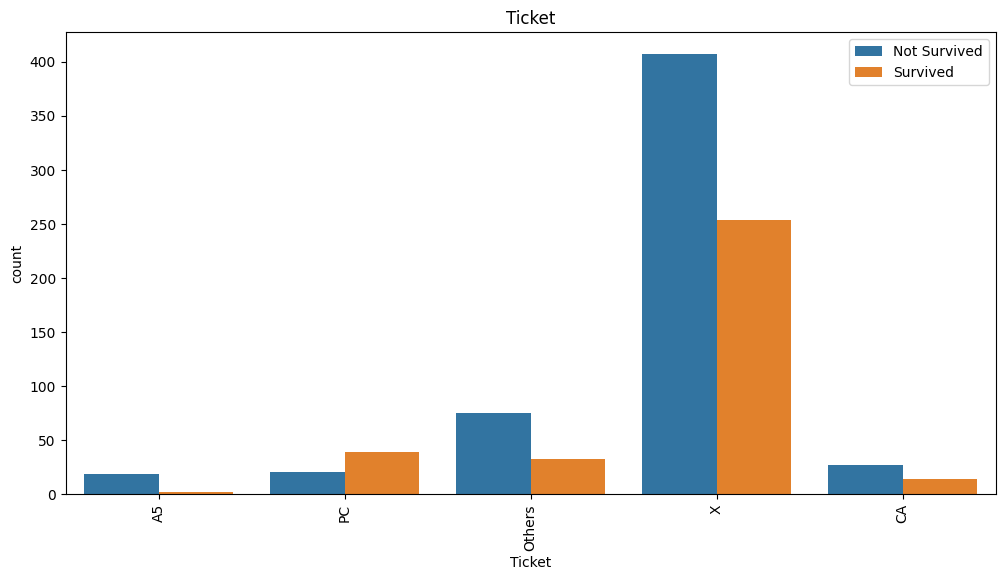
\includegraphics[width=\columnwidth]{titanicreport/figs/fig9.png}
    \caption{Tỷ lệ sống sót của hành khách trên tàu Titanic theo loại vé.}
    \label{fig:ticket}
\end{figure}
% Example:
Mặt khác, chúng tôi nhận thấy trong bộ Dataset, có 2 cột liên quan tới gia đình là \textbf{Sibsp} và \textbf{Parch}. Đầu tiên, chúng tôi tạo một đặc trưng mới 'Family Size' bằng cách  gộp hai cột SibSp (số lượng anh chị em hoặc vợ chồng đi cùng) và Parch (số lượng cha mẹ hoặc con cái đi cùng) thành một cột mới, thể hiện tổng số lượng thành viên trong gia đình đi cùng trên tàu.Family Size là một đặc trưng tổng quát và dễ hiểu hơn về kích thước của gia đình. Thay vì xem xét riêng lẻ \textbf{Sibsp} và \textbf{Parch}, việc kết hợp chúng thành một đặc trưng gia đình có thể giúp mô hình học máy hiểu được mối quan hệ tổng thể giữa kích thước gia đình và khả năng sống sót. Điều này có thể giúp giảm số lượng đặc trưng, làm cho mô hình trở nên dễ quản lý hơn và có thể cải thiện hiệu suất của mô hình.Family Size: Số lượng thành viên trong gia đình của mỗi hành khách sẽ dao động từ 1 đến 11.\\
\begin{figure}[ht]
    \centering
    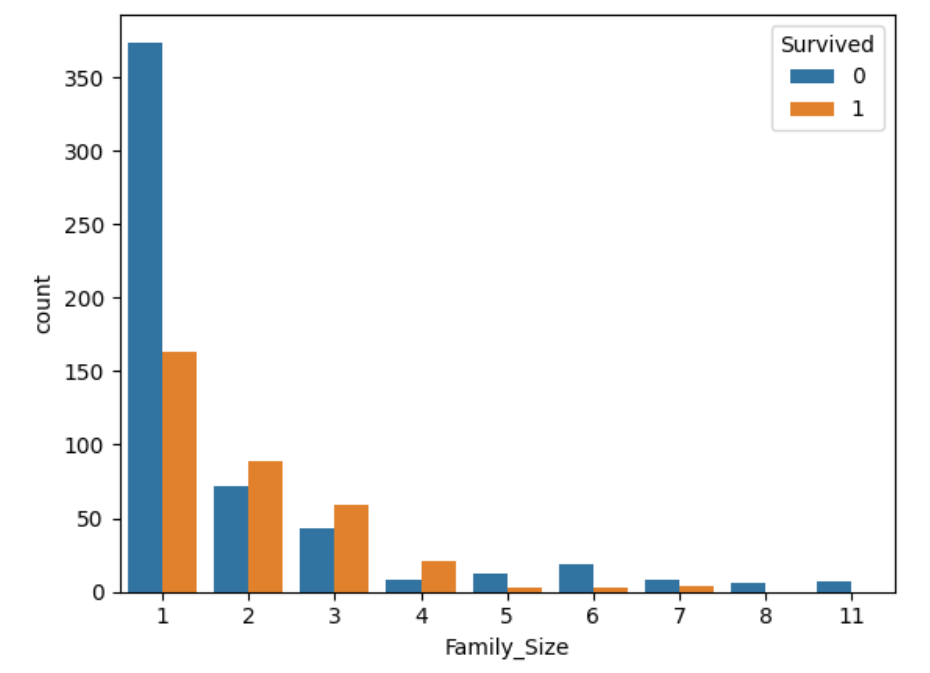
\includegraphics[width=\columnwidth]{titanicreport/figs/family_size.png}
    \caption{Số lượng thành viên trong gia đình của mỗi hành khách.}
\end{figure}
Tiếp theo, chúng tôi phân loại gia đình của mỗi hành khách dựa vào đặc trưng Family Size mới tạo. Family Cat: Loại gia đình của mỗi hành khách sẽ được phân loại thành một trong bốn loại sau:
\begin{itemize}
    \item Single: Hành khách đi một mình.
    \item Small: Hành khách đi cùng 1-4 thành viên trong gia đình.
    \item Medium: Hành khách đi cùng 5-7 thành viên trong gia đình.
    \item Large: Hành khách đi cùng 8-11 thành viên trong gia đình.     
\end{itemize}
\begin{figure}[ht]
    \centering
    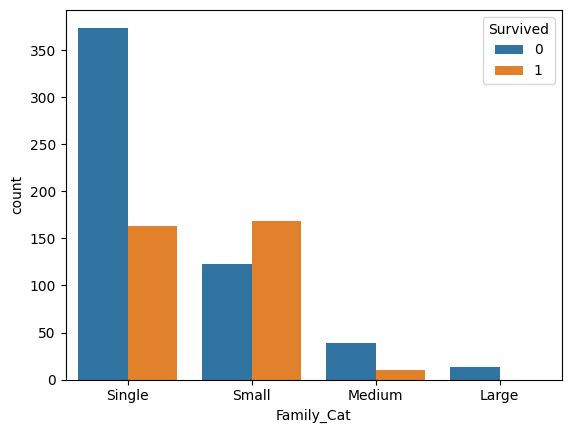
\includegraphics[width=\columnwidth]{titanicreport/figs/family_cat.png}
    \caption{Loại gia đình của mỗi hành khách.}
    \label{fig:family_cat}
\end{figure}
Biểu đồ hình~\ref{fig:family_cat} hiển thị phân phối tỷ lệ sống sót của hành khách trên tàu Titanic theo kích thước gia đình. Có thể thấy rằng tỷ lệ sống sót của hành khách đi một mình cao hơn đáng kể so với tỷ lệ sống sót của hành khách đi cùng gia đình lớn. Cụ thể, tỷ lệ sống sót của hành khách đi một mình là 38,5\%, cao hơn tỷ lệ sống sót của hành khách đi cùng gia đình nhỏ (29,2\%), gia đình trung bình (22,5\%) và gia đình lớn (20,1\%).
Biểu đồ này cung cấp một số thông tin quan trọng về mối quan hệ giữa kích thước gia đình và tỷ lệ sống sót. Thông tin này được sử dụng để hiểu rõ hơn về thảm họa Titanic và để phát triển các mô hình học máy hiệu quả hơn để dự đoán khả năng sống sót của hành khách.
Ngoài ra, chúng tôi nhận thấy, có rất nhiều gia đình loại Single Family, cho nên chúng tôi tạo một feature mới 'Alone' đại diện cho người đi tàu một mình. Biểu đồ hình ~\ref{fig:family_cat} hiển thị phân phối tỷ lệ sống sót của hành khách trên tàu Titanic theo biến "Alone". Biến này có hai giá trị:
\begin{itemize}
    \item 0: Hành khách không đi một mình.
    \item 1: Hành khách đi một mình.
\end{itemize}
Biểu đồ cho thấy rằng tỷ lệ sống sót của hành khách đi một mình thấp hơn đáng kể so với tỷ lệ sống sót của hành khách không đi một mình. Cụ thể, tỷ lệ sống sót của hành khách đi một mình là 38,5\%, thấp hơn tỷ lệ sống sót của hành khách không đi một mình là 62,5\%.\\
\begin{figure}[ht]
    \centering
    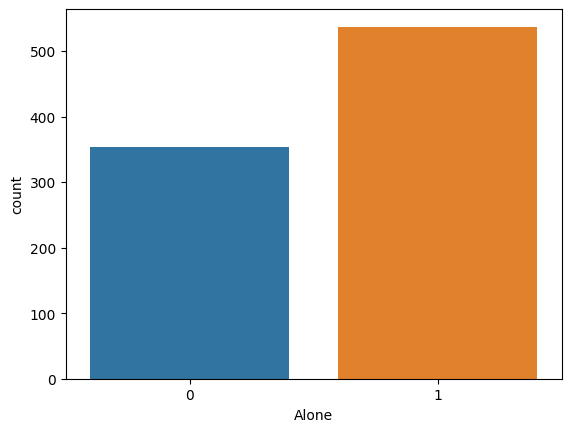
\includegraphics[width=\columnwidth]{titanicreport/figs/Alone.png}
    \caption{Số lượng hành khách đi một mình.}
    \label{fig:Alone}
\end{figure}
Cuối cùng, 
\subsection{Data Wrangling}
Trong quá trình chuẩn bị và làm sạch dữ liệu, việc xử lý giá trị thiếu là một bước quan trọng để đảm bảo tính chính xác và đồng nhất của dữ liệu. Đầu tiên, chúng tôi dùng hàm 'missing display' để hiển thị thông tin về giá trị thiếu trong các đặc trưng của DataFrame. Ở tập huấn luyện (train) ta thấy feature 'Age' có 19.87\% giá trị thiếu, 'Embarked' có 0.22\% giá trị thiếu. Đối với tập kiểm thử(test), feature Age' có 20.57\% giá trị thiếu, 'Fare' có 0.24\% giá trị thiếu. Tiếp theo chúng tôi sẽ dùng hai phương pháp để xử lý giá trị thiếu: Simple Imputer từ thư viện scikit-learn và missForest từ thư viện missingpy.

\subsubsection{Use Simple Imputer}
Sử dụng \textbf{Simple Imputer} từ sklearn để fill missing data, Sử dụng chiến lược 'median' để điền giá trị thiếu cho numerical data. Áp dụng chuẩn hóa dữ liệu bằng StandardScaler để đồng nhất đơn vị đo và phân phối.Đối với categorical data là mean và most frequent ~\ref{fig:skimputer}. Dữ liệu từ bước trước là một mảng NumPy, và bước này tạo một DataFrame mới từ mảng này. Các cột được đặt tên dựa trên danh sách num features và cat features. Tiếp đến, chuyển đổi đặc trưng categorical thành dạng số. Sau đó tiến hành các bước chuyển đổi kiểu dữ liệu của một số cột trong DataFrame. Việc này giúp đảm bảo rằng dữ liệu đã được chuẩn bị có kiểu dữ liệu phù hợp cho việc đưa vào mô hình học máy. Điều này có thể là quan trọng vì mô hình yêu cầu kiểu dữ liệu chính xác để thực hiện các phép toán một cách đúng đắn. Biểu đồ heatmap Figure~\ref{fig:heatmap} này thường được sử dụng để kiểm tra mối quan hệ tương quan giữa các đặc trưng.\\
\begin{figure}[ht]
    \centering
    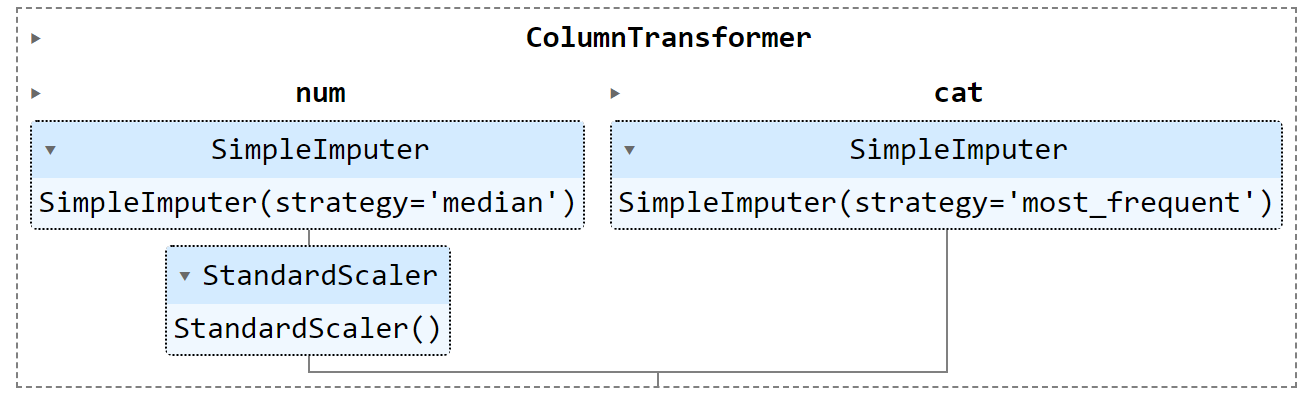
\includegraphics[width=\columnwidth]{titanicreport/figs/skimputer.png}
    \caption{Sklearn Imputer Pipeline.}
    \label{fig:skimputer}
\end{figure}
\begin{figure}[ht]
    \centering
    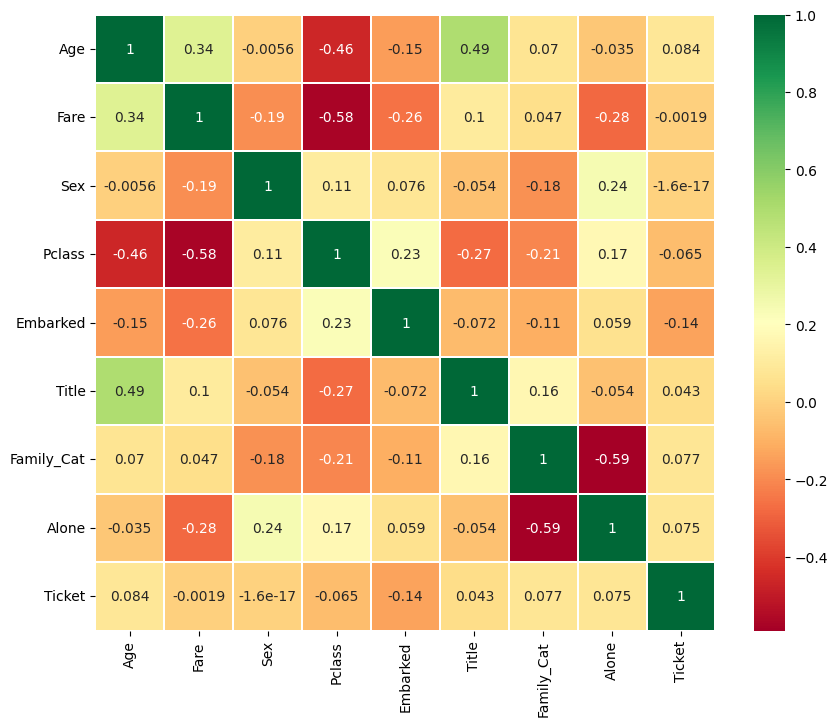
\includegraphics[width=\columnwidth]{titanicreport/figs/corr_matrix_1.png}
    \caption{Ma trận tương quan sau khi preprocess}
    \label{fig:heatmap}
\end{figure}
Tiếp theo, chúng tôi tiến hành chia tập dữ liệu, đây là một bước quan trọng trong quá trình xây dựng mô hình học máy. Trong bộ dữ liệu này chúng tôi chia thành hai phần: một phần để huấn luyện mô hình và một phần để kiểm tra hiệu suất của mô hình trên dữ liệu mới mà nó chưa từng thấy.\\
Cuối cùng, tiến hành huấn luyện và đánh giá mô hình.
\begin{table}[htbp]
\centering
\caption{Kết quả đánh giá hiệu suất của các mô hình}
\label{tab:model_evaluation}
\begin{tabular}{|l|r|}
\hline
\textbf{Model Name} & \textbf{Mean} \\
\hline
GradientBoostingClassifier & 0.835550 \\
SVC & 0.834220 \\
AdaBoostClassifier & 0.825857 \\
XGBClassifier & 0.821395 \\
LinearSVC & 0.814509 \\
RandomForestClassifier & 0.811525 \\
LogisticRegression & 0.808924 \\
DecisionTreeClassifier & 0.805999 \\
KNeighborsClassifier & 0.801773 \\
ExtraTreesClassifier & 0.797547 \\
\hline
\end{tabular}
\end{table}
 Hình ~\ref{fig: Accuracy}  là kết quả đánh giá hiệu suất trung bình của các mô hình học máy trên dữ liệu huấn luyện sử dụng phương pháp cross-validation. 
\begin{figure}[ht]
    \centering
    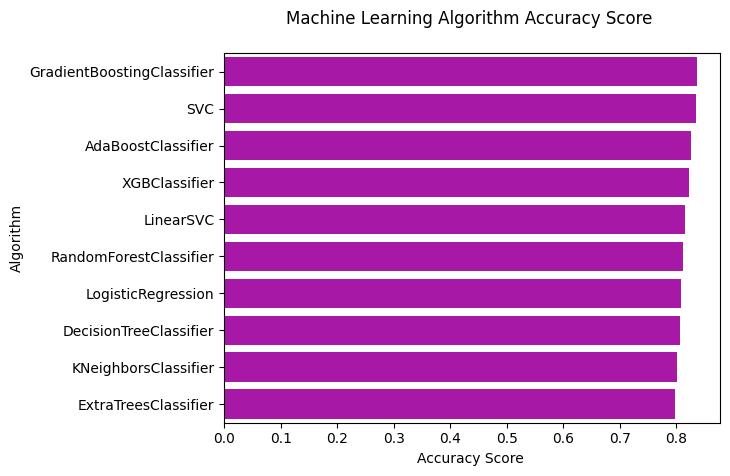
\includegraphics[width=\columnwidth]{titanicreport/figs/Accuracy.png}
    \caption{Độ chính xác của các mô hình học máy}
    \label{fig: Accuracy}
\end{figure}
\subsubsection{ Use Missingpy}
Sử dụng thư viện Missingpy là một công cụ mạnh mẽ và linh hoạt trong việc xử lý dữ liệu thiếu bằng cách train những feature còn lại. Tích hợp mượt mà với scikit-learn, thư viện cung cấp nhiều thuật toán điền giá trị, trong đó có MissForest được sử dụng trong đồ án này. Với khả năng xử lý cả biến phân loại và liên tục, missingpy mang lại tính nhất quán và đồng bộ trong các quy trình học máy và xử lý dữ liệu. Sự linh hoạt và khả năng tùy chỉnh của thư viện làm cho nó trở thành một công cụ hữu ích trong việc chuẩn bị dữ liệu cho mô hình học máy. \\
Đầu tiên, chúng tôi sử dụng LabelEncoder để chuyển đổi các biến dạng chuỗi trong các cột phân loại thành các số nguyên. Tiếp theo, tạo một đối tượng MissForest với các tham số cụ thể: 'squared\_error': sử dụng tiêu chí bình phương lỗi để ước lượng giá trị thiếu. Áp dụng thuật toán MissForest và điền giá trị thiếu cho cả train data và test data. Qua đó, các giá trị thiếu trong dữ liệu đã được ước lượng và điền vào, giúp chuẩn bị dữ liệu cho quá trình huấn luyện mô hình học máy một cách đầy đủ. Sau khi áp dụng MissForest, tiến hành chuyển đổi chúng từ các mảng Numpy thành DataFrame của pandas. 

\begin{figure}[ht]
    \centering
    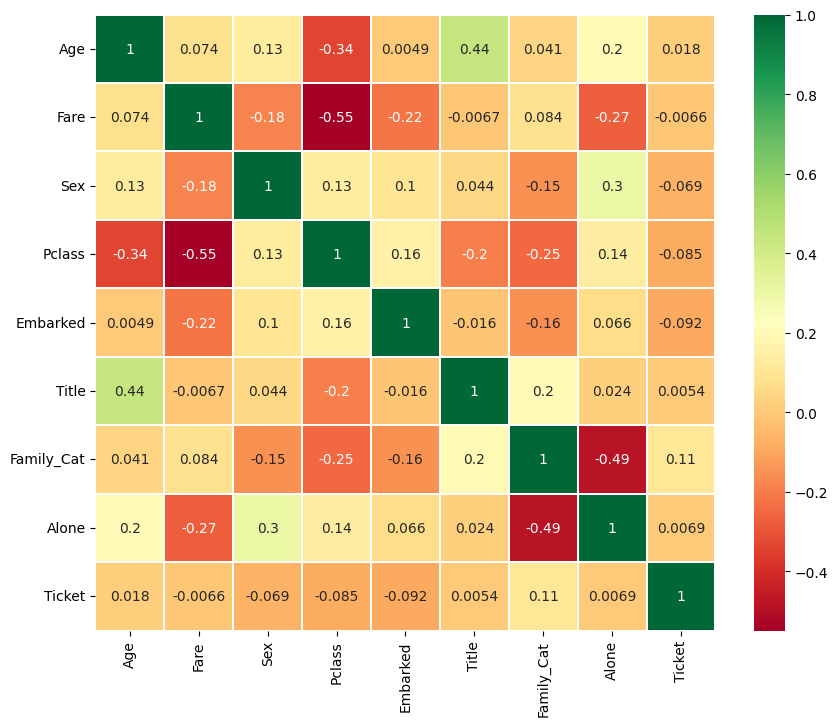
\includegraphics[width=\columnwidth]{titanicreport/figs/corr_matrix_2.png}
    \caption{Ma trận tương quan sau khi preprocess}
\end{figure}
Bảng ~\ref{tab: missingpy} là kết quả đánh giá hiệu suất trung bình của các mô hình học máy trên dữ liệu huấn luyện sử dụng phương pháp cross-validation. 
\begin{table}[htbp]
\centering
\caption{Kết quả đánh giá hiệu suất của các mô hình}
\label{tab: missingpy}
\begin{tabular}{|l|r|}
\hline
\textbf{Model Name} & \textbf{Mean} \\
\hline
\text{GradientBoostingClassifier} & 0.777513 \\
\text{LinearSVC} & 0.767901 \\
\text{KNeighborsClassifier} & 0.765520 \\
\text{XGBClassifier} & 0.763316 \\
\text{LogisticRegression} & 0.763228 \\
\text{SVC} & 0.763139 \\
\text{ExtraTreesClassifier} & 0.758466 \\
\text{RandomForestClassifier} & 0.758377 \\
\text{DecisionTreeClassifier} & 0.746120 \\
\text{AdaBoostClassifier} & 0.734392 \\
\hline
\end{tabular}
\end{table}

\section{Feature \& Model Selection}
 Chúng tôi dùng 10 mô hình học máy: Logistic Regression,Linear Support Vector Classification (LinearSVC), Support Vector Classification (SVC), K-Nearest Neighbors (KNN), Decision Tree Classifier, Random Forest Classifier, Extra Trees Classifier, AdaBoost Classifier, XGBoost Classifier,,Gradient Boosting Classifier. Việc sử dụng 10 mô hình học máy khác nhau mang lại nhiều lợi ích. Điều này giúp so sánh hiệu suất, tìm kiếm siêu tham số tối ưu, và đảm bảo tính đồng nhất trong dự báo. Việc khám phá và hiểu rõ mỗi mô hình trở nên dễ dàng, cùng việc đối phó với độ phức tạp đa dạng trong dữ liệu. Sử dụng nhiều mô hình làm tăng khả năng kiểm soát overfitting và underfitting. Cuối cùng, cơ hội để thử nghiệm các kỹ thuật như stacking giúp tạo ra một mô hình mạnh mẽ và ổn định. Đây là bài toán binary classification, dựa trên sklearn model selection ( hình~\ref{fig: scikit}) nhóm thực hiện chạy thử và so sánh các model phù hợp với bài toán. Sử dụng StratifiedKFold của model selection để chọn ra 5-6 model tốt nhất.  
\begin{figure}[ht]
    \centering
    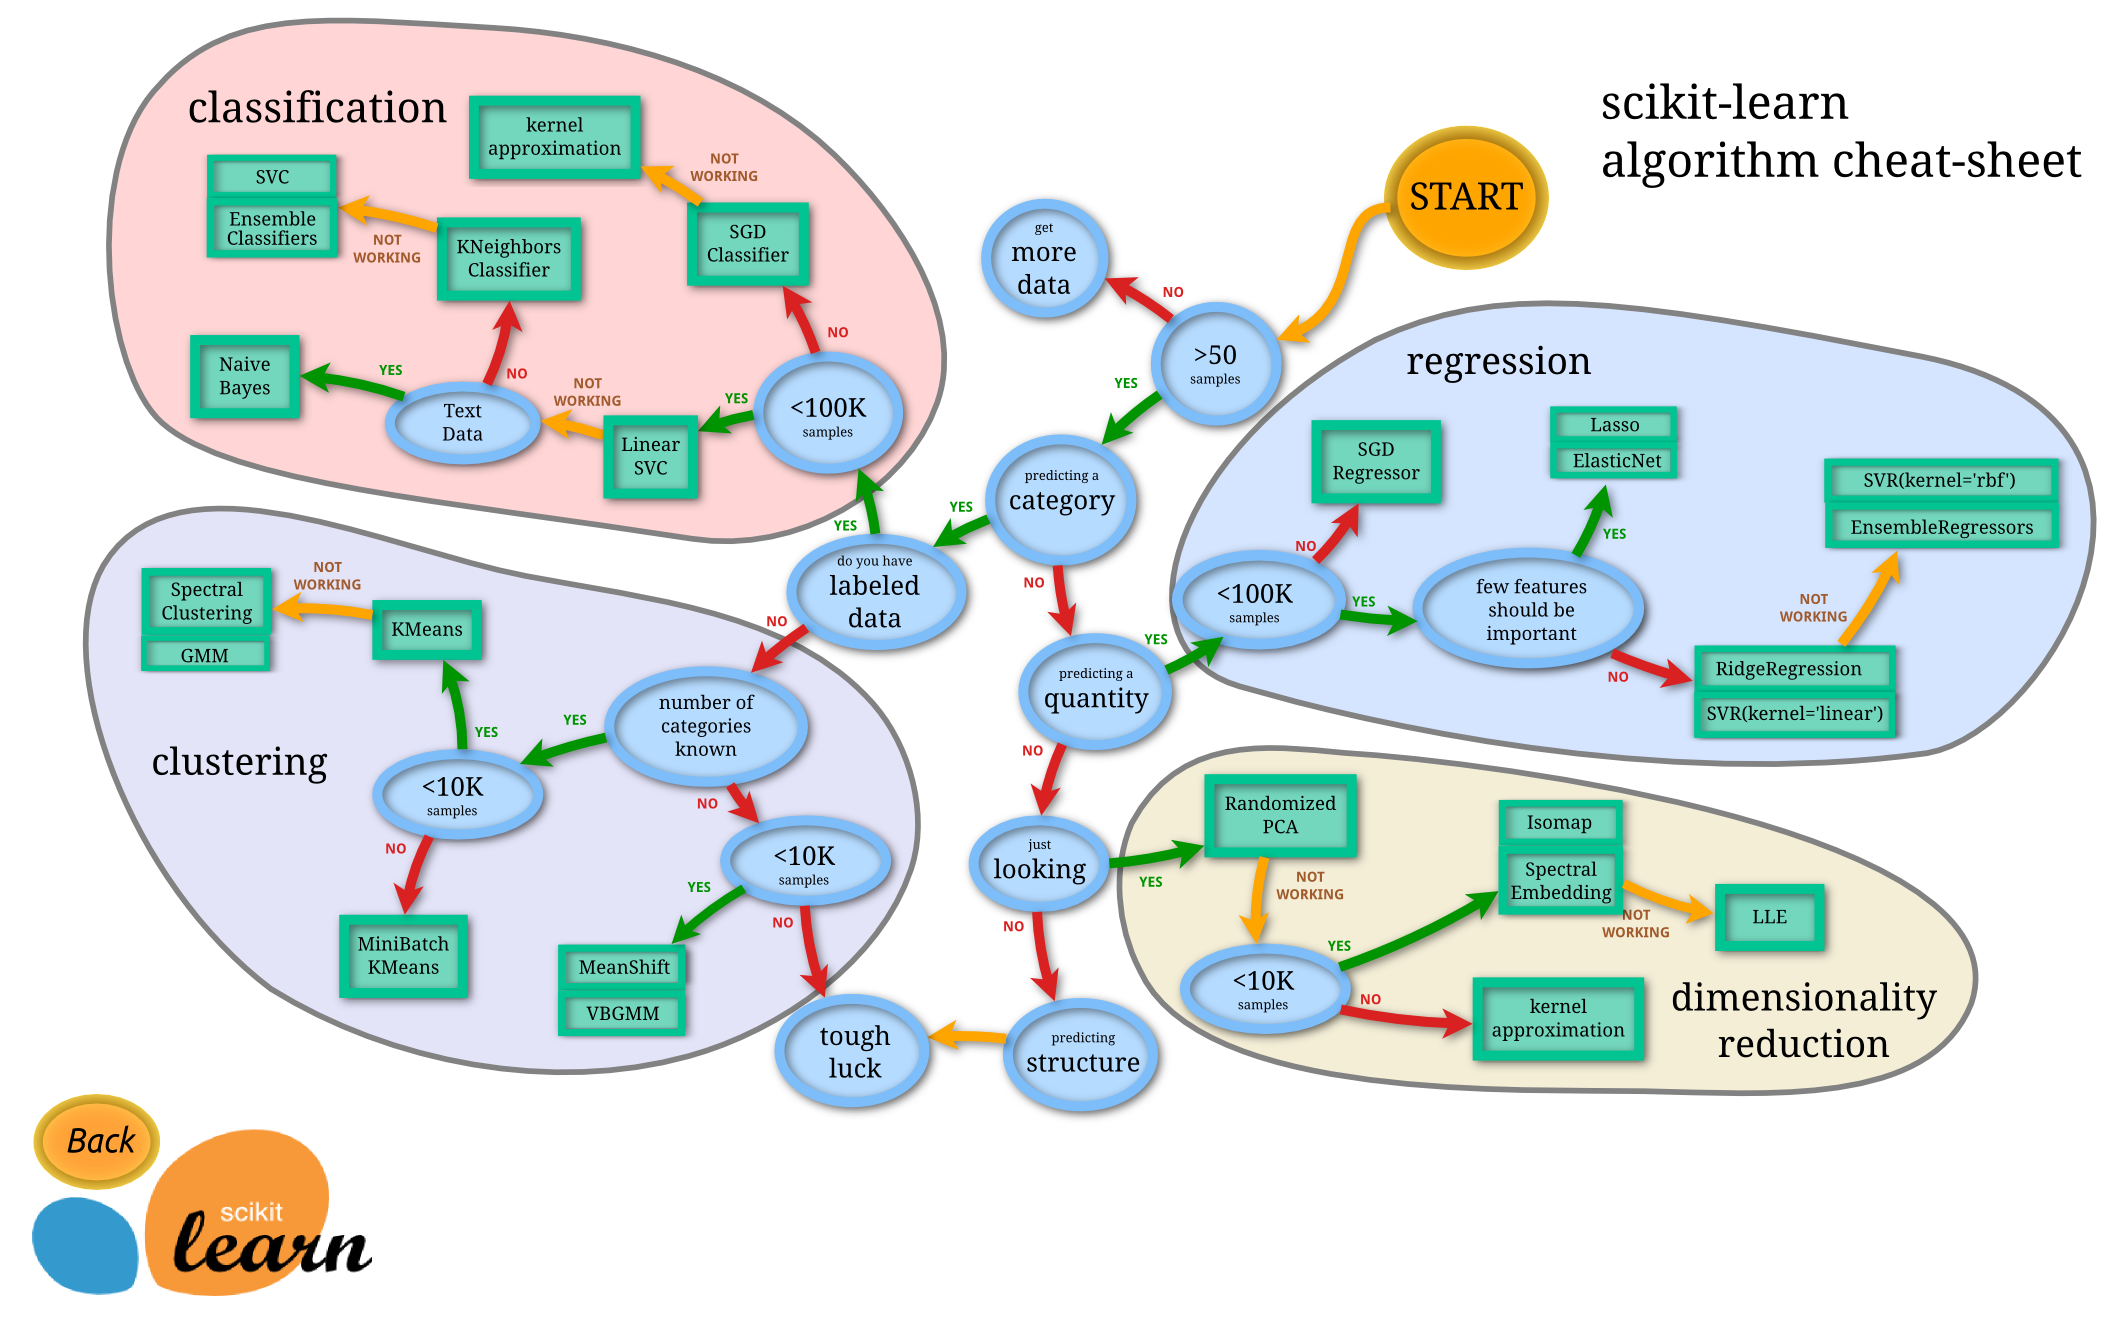
\includegraphics[width=\columnwidth]{titanicreport/figs/scikit.png}
    \caption{Sklearn model selection }
    \label{fig: scikit}
\end{figure}


Qua đó, chúng tôi đã chọn được các mô hình tốt nhất. Cụ thể là: GradientBoostingClassifier, SVC (Support Vector Classification), AdaBoostClassifier, RandomForestClassifier, XGBClassifier, DecisionTreeClassifier. Cuối cùng, chúng tôi tiến hành huấn luyện, tinh chỉnh và đánh giá tập dữ liệu theo mô hình Gradient Boosting Classifier.
\section{Result \& Discussion}
Sau khi tiến hành huấn luyện và đánh giá mô hình, chúng tôi nhận thấy mô hình Gradient Boosting Classifier đạt kết quả tốt nhất. Vì vậy, nhóm quyết định sử dụng mô hình này để huấn luyện và dự đoán đự đoán.\\
Bảng \ref{tab:gradient_boosting_results} là kết quả đánh giá hiệu suất của mô hình Gradient Boosting Classifier khi sử dụng thư viện Missingpy xử lý dữ liệu thiếu của tập dữ liệu Titanic.\\
\begin{table}[htbp]
\centering
\caption{Gradient Boosting Classifier Performance Evaluation}
\label{tab:gradient_boosting_results}
\begin{tabular}{|l|l|l|l|}
\hline
\textbf{} & \textbf{Precision} & \textbf{Recall} & \textbf{F1-score}  \\ \hline
\textbf{0} & 89\%&96\%&92\%\\ \hline 
\textbf{1} & 88\%&72\%&79\%\\ \hline 
\textbf{Accuracy} & &  & 89\%  \\ \hline
\textbf{Macro Avg} & 89\% & 84\% & 86\%  \\ \hline
\textbf{Weighted Avg} & 89\% & 89\% & 88\%  \\ \hline
\end{tabular}
\end{table}
So với sử dụng \textbf{Missingpy} từ sklearn để fill missing data thì \textbf{Simple Imputer} cho độ chính xác cũng như hiệu suất của mô hình thấp hơn đáng kể. 
\begin{table}[htbp]
\centering
\caption{Hiệu suất mô hình Gradient Boosting Classifier khi dùng Simple Imputer}
\label{tab:simple}
\begin{tabular}{|l|l|l|l|}
\hline
\textbf{} & \textbf{Precision} & \textbf{Recall} & \textbf{F1-score} \\ \hline
\textbf{0} & 81\% & 81\% & 81\% \\ \hline 
\textbf{1} & 69\% & 70\% & 69\% \\ \hline 
\textbf{Accuracy} & & & 77\% \\ \hline
\textbf{Macro Avg} & 75\% & 75\% & 75\% \\ \hline
\textbf{Weighted Avg} & 77\% & 77\% & 77\% \\ \hline
\end{tabular}
\end{table}


\section{Conclusion}
     \textbf{Kết luận:}  Dự án này không chỉ giúp hiểu rõ hơn về các đặc trưng quyết định sống sót trên tàu Titanic mà còn thể hiện quá trình triển khai mô hình học máy để dự đoán trong tình huống tương tự. Việc sử dụng mô hình học máy phức tạp và kỹ thuật tiền xử lý thông minh có thể cải thiện khả năng dự đoán, mang lại hiệu suất đáng kể trong việc dự đoán sống sót.\\
     \textbf{Học được:} Trong quá trình thực hiện dự án, chúng tôi đã có cơ hội áp dụng kiến thức lý thuyết, học được cách xử lý dữ liệu thiếu, chọn mô hình phù hợp và điều chỉnh tham số để cải thiện hiệu suất.\\
     \textbf{Hướng Phát Triển:}
  Dự án mở ra nhiều khả năng phát triển, từ việc thêm các đặc trưng mới đến thử nghiệm với các mô hình phức tạp hơn để nâng cao độ chính xác.

\begin{thebibliography}{9}

\bibitem{dataset_ref}
    Titanic: Machine Learning from Disaster Dataset,
    \textit{Kaggle},
    \url{https://www.kaggle.com/c/titanic/data}

\bibitem{scikit-learn_ref}
    Pedregosa, F., Varoquaux, G., Gramfort, A., Michel, V., Thirion, B., Grisel, O., ... \& Vanderplas, J.
    \textit{Scikit-learn: Machine Learning in Python},
    \url{https://scikit-learn.org/stable/}

\bibitem{missingpy_ref}
    MissForest Documentation,
    \textit{GitHub},
    \url{https://github.com/epsilon-machine/missingpy}

\bibitem{scikit-learn_estimator_guide}
    Choosing the right estimator,
    \textit{Scikit-learn Documentation},
    \url{https://scikit-learn.org/stable/tutorial/machine_learning_map/index.html}


\bibitem{matplotlib_ref}
    Hunter, J. D.
    \textit{Matplotlib: A 2D Graphics Environment},
    \url{https://matplotlib.org/}

\end{thebibliography}


\end{document}
